This chapter describes the implementation of the cached profiles implementation for Hotspot, written as part of this thesis.
\\\\
Hotspot is an Java virtual machine implementation maintained by Oracle Cooperation. It is part of the open source project \texttt{OpenJDK} and the source code is available at \url{http://openjdk.java.net/}.
\\\\
Most of the work is included in two new classes \texttt{/share/vm/ci/ciCacheProfiles.cpp} and \\\texttt{/share/vm/ci/ciCacheProfilesBroker.cpp} as well as modifications to \texttt{/share/vm/ci/ciEnv.cpp} and \texttt{/share/vm/compiler/compileBroker.cpp}.
\\
Most of the code is located in \texttt{/share/vm/ci/ciCacheProfiles.cpp}, a class that takes care of setting up a datastructure for the cached profiles as well as providing public methods to check if a method is cached or not. The class \texttt{/share/vm/ci/ciCacheProfilesBroker.cpp} gets called before a method that has a profile available gets compiled. It is responsible for setting up the compilation environment so the JIT compiler can use the cached profiles.
\\\\
A full list of modified files and the changes can be seen in the webrev or appendix TODO.
\\\\
The changes are provided in form of a patch for Hotspot version 8182 TODO. This original version is referred to as \textit{Baseline}.
\\\\
I will describe and explain the functionality and the implementation design decision in the following sections, ordered by the appearance in execution.


\section{Creating cached profiles}
\label{s:creatingprofiles}
The baseline version of Hotspot already offered a functionality to replay a compilation based on dumped profiling information.
This is mainly used in case the JVM crashes during JIT compilation to replay the compilation again and help finding the cause of this crash.
Dumping the data needed for the replay is either be done automatically in case of a crash or can be invoked manually by specifying the \texttt{DumpReplay} compile command option per method.
I introduce method option called \texttt{DumpProfile} as well as a compiler flag \texttt{-XX:+DumpProfiles} that appends profiling information to a file as soon as the method gets compiled. The first option can be specified as part of the \texttt{-XX:CompileCommand} or \texttt{-XX:CompileCommandFile} flag and allows one to force single methods to dump their profile. The second commands dumps all profiles of all compiled methods into a single file called \textit{cached\_profiles.dat}.
\\\\
As soon as a method gets compiled all information about the methods used in the compiled method as well as their profiling information get converted to a string and written to disk. Since method often get compiled multiple times this can result in dumping compilation information about the same method multiple times. How this will be taken care of is described in Section \ref{s:initializingprofiles}
Together with some additional information about the compilation itself, for example the bytecode index of the compiled method in case of OSR, the compiler will be able to redo the same compilation on a future run of the java virtual machine.  
\section{Initializing cached profiles}
\label{s:initializingprofiles}
I introduce a new compiler flag \texttt{-XX:+CacheProfiles} that enables the use of profiles that have been written to disk in a previous run of the Java Virtual Machine. Per default it reads from a file called \textit{cached\_profiles.dat} but a different file can be specified using \\\texttt{-XX:CacheProfilesFile=other\_file.dat}.
\\\\
Before any cached profiles can be used the virtual machine has to parse that file and organize the profiles and compile information in a simple datastructure. This datastructure is kept in memory during the whole execution of the JVM to avoid multiple scans of the file.
The parsing process gets invoked during boot up of the JVM, directly after the compileBroker gets initialized. This happens before any methods get executed and blocks the JVM until finished.
As mentioned in Section \ref{s:creatingprofiles} the file consists of method informations, method profiles and additional compile information. The parser scans the file once and creates a so called \texttt{CompileRecord} for each of the methods that include compilation information in the file. This compile record also includes the list of method information and their profiling information.
A method's compile information could have been dumped multiple times, so it can happen that there are multiple CompileRecords for the same method. In this case, Hotspot will only keep the CompileRecords that are created based on the data written to the file last.
Since profiling information only grow, the compilation that happened last contains the richest profile and is considered the best to avoid deoptimizations.
\\\\
The CompileRecord as well as the lists of methods information and profiles are implemented as an array located in Hotspot's heap space.
They get initialized with a length of 8 and grow when needed. The choice has been done for simplicity and leaves up room for further optimizations.

\section{Using cached profiles}
\label{s:usingprofiles}
The idea is to use cached profiles whenever possible and if none are available continue as usual.
A graphical, simplified overview of the program flow for compiling a method with the changes introduced in this thesis can be found in Figure \ref{f:programflow}.
\begin{figure}[h]
  \begin{center}
    \centering
    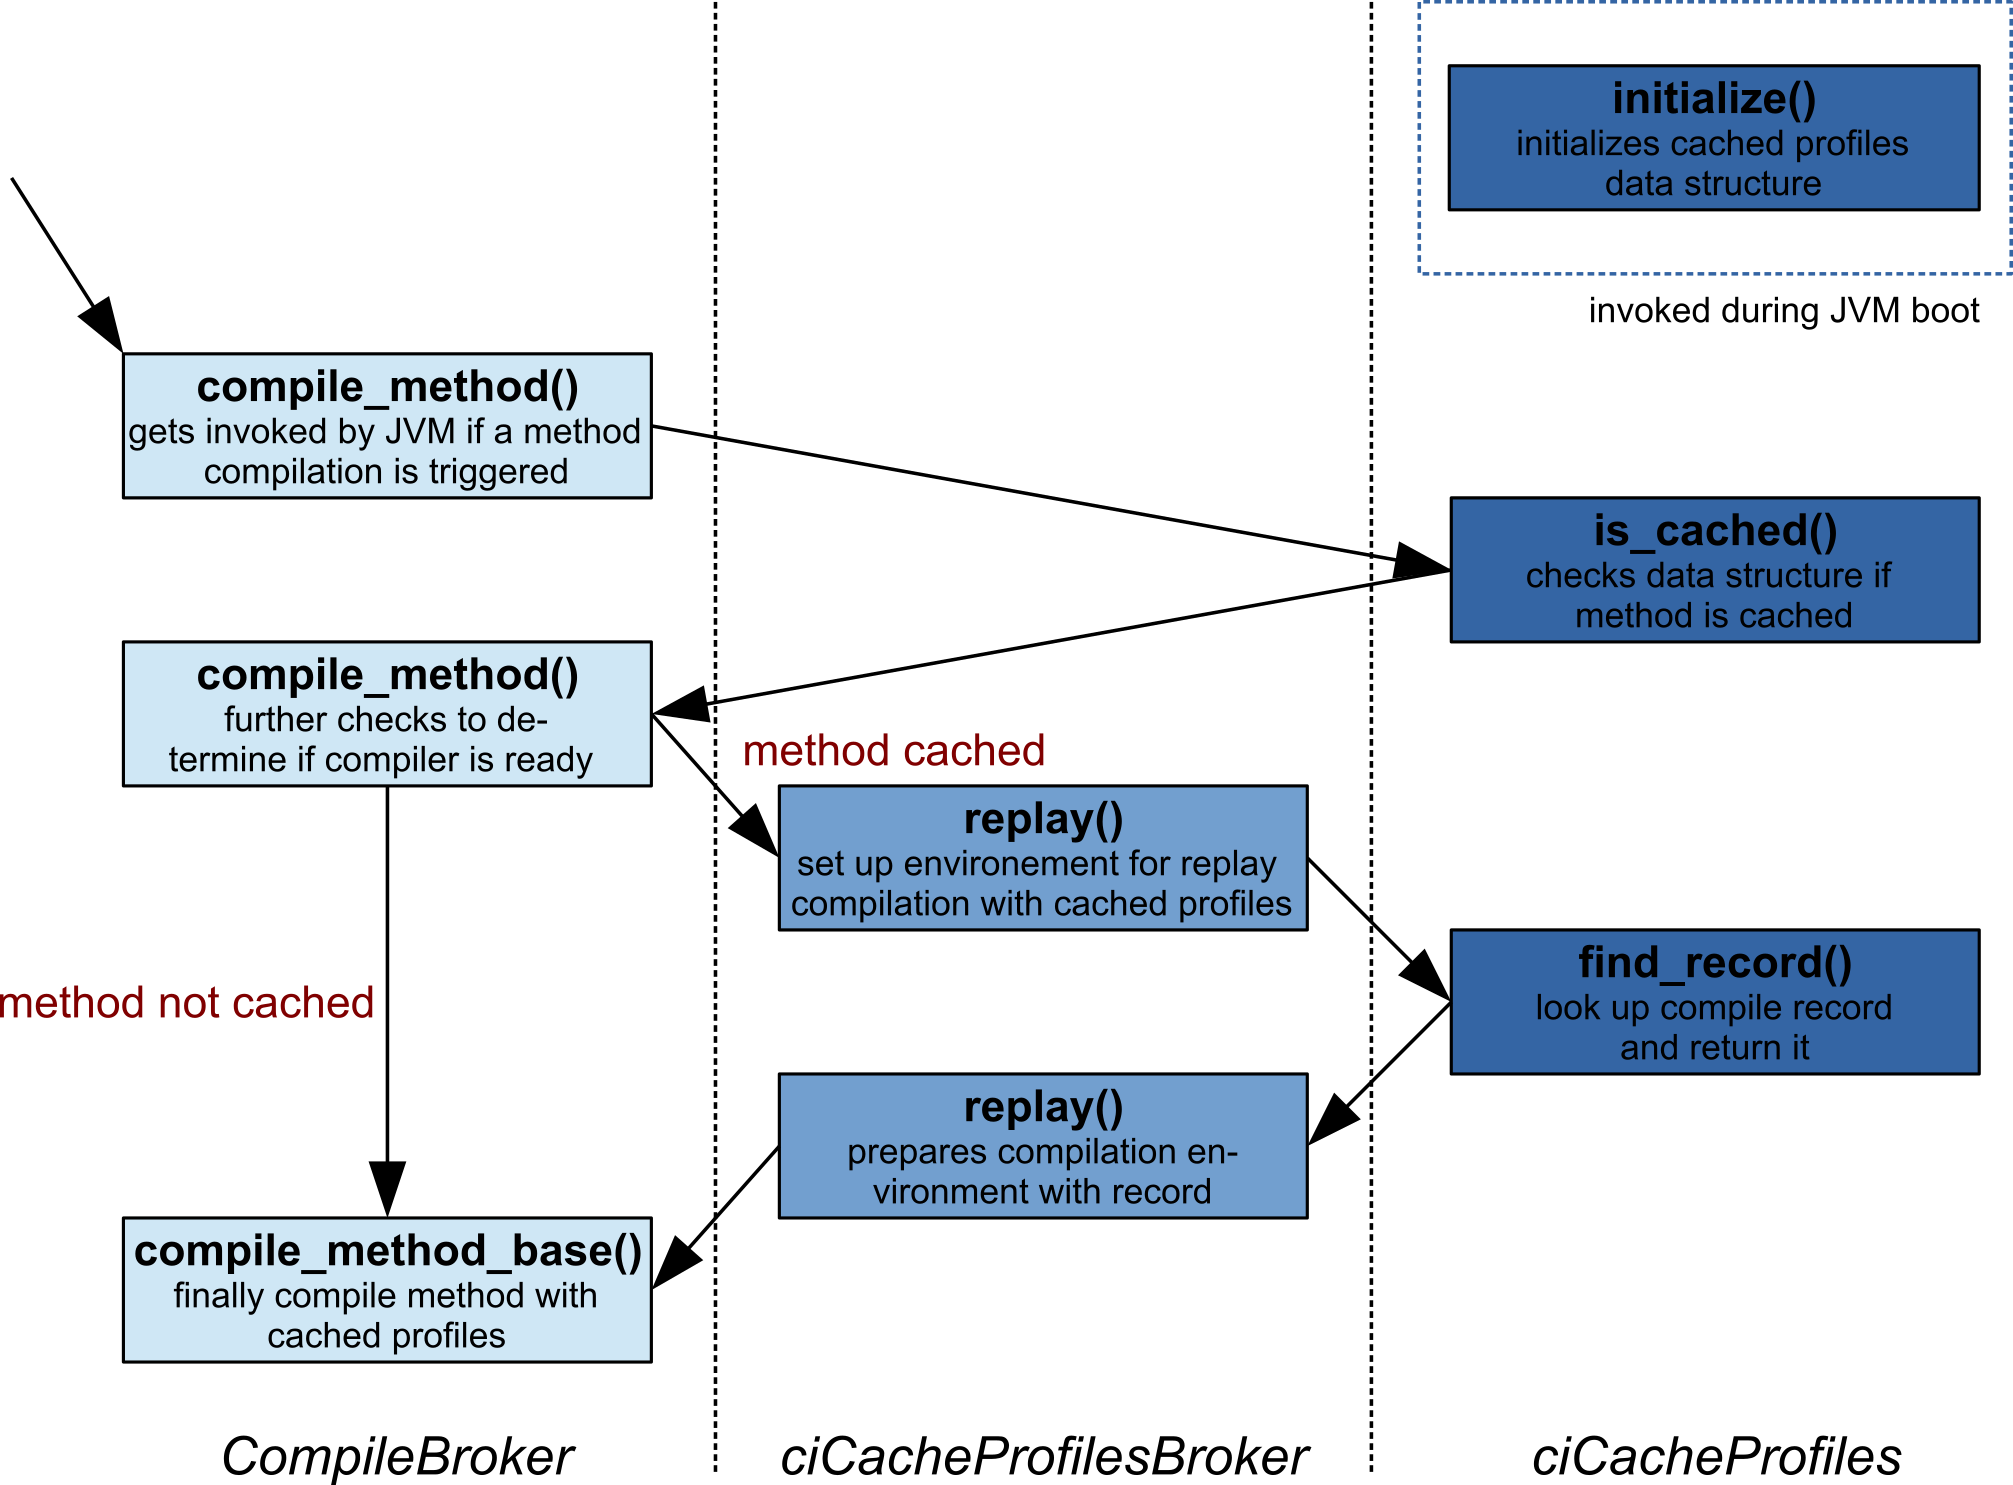
\includegraphics[width=0.8\textwidth]{figures/program_flow.png}
    \caption{program flow for compiling a method}
    \label{f:programflow}
  \end{center}
\end{figure}
As mentioned before once certain thresholds are exceeded a method gets scheduled for compilation. This means that the JVM will invoke a method called \texttt{compile\_method()} located in the \texttt{compileBroker} class. This method for example checks if the compile queue isn't full or if there is already another compilation of that particular method running.
I extended this method with a call to \texttt{ciCacheProfiles::is\_cached(Method* method)} which either returns 0 if the method is not cached or returns an integer value, reflecting the compile level, in case that method has a cached profile available.
In case the method is not cached the execution continues as in the baseline.
Otherwise the compileBroker will call into \texttt{ciCacheProfilesBroker} to replay the compilation, based on the saved profile.

\section{Different usage modes for cached profiles}
The implementation of cached profiles offers 3 different modes which differ 
\begin{figure}[h]
  \begin{center}
    \centering
    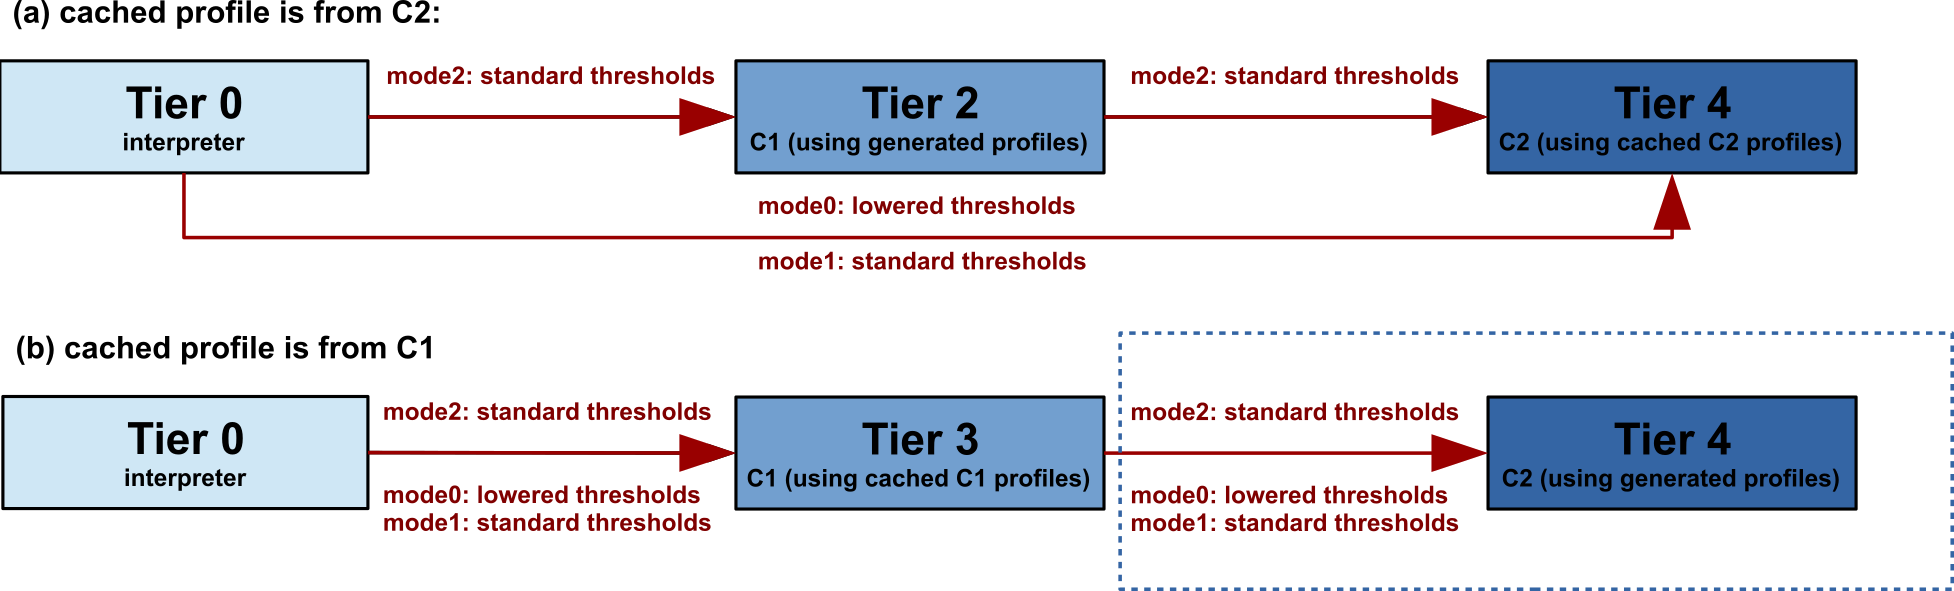
\includegraphics{figures/hs_tiers_threshold.png}
    \caption{Overview over compilation tiers with different modes}
    \label{f:hs_tiers_thresholds}
  \end{center}
\end{figure}

\label{s:cacheprofilesmode}
\subsection{Compile Thresholds lowered (mode 0)}
\label{s:mode0}
\subsection{Unmodified Compile Thresholds (mode 1)}
\label{s:mode1}
\subsection{Modified C1 stage (mode 2)}
\label{s:mode2}

\section{Debug output}
\label{s:debugoutput}
For debugging and benchmarking purposes I implemented four debug flags that can be used along with \texttt{-XX:+CacheProfiles}.
\begin{table}[ht]
  \centering
 % \caption{}
  \label{t:debugflags}
  \begin{center}
    \begin{tabular}{| l | p{9.0cm} |}
       \hline
       \textbf{flag} & \textbf{description} \\ \hline\hline
       -XX:+PrintCacheProfiles & enable command line debug output for cached profiles\\ \hline
       -XX:+PrintDeoptimizationCount & prints amount of deoptimizations when the JVM gets shut down\\ \hline
       -XX:+PrintDeoptimizationCountVerbose & prints total the amount of deoptimizations on each deoptimization\\ \hline
       -XX:+PrintCompileQueue & prints the total amount of methods in the compile queue each time a method gets added \\ \hline
    \end{tabular}
  \end{center}
\end{table}



